

\tikzset{every picture/.style={line width=0.75pt}} %set default line width to 0.75pt        

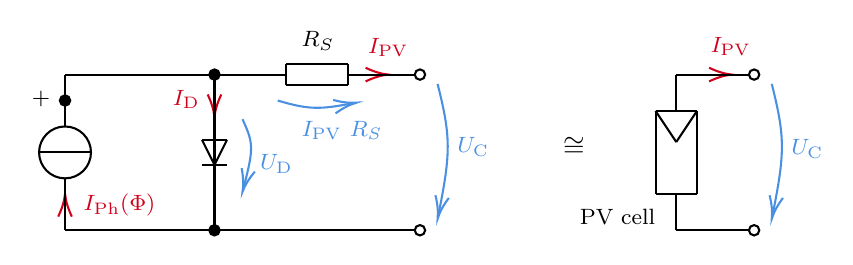
\begin{tikzpicture}[x=0.75pt,y=0.75pt,yscale=-1,xscale=1]
%uncomment if require: \path (0,391); %set diagram left start at 0, and has height of 391

%Straight Lines [id:da4539360054023531] 
\draw [color={rgb, 255:red, 208; green, 2; blue, 27 }  ,draw opacity=1 ]   (402,152.5) -- (415.75,152.5) ;
\draw [shift={(417.75,152.5)}, rotate = 180] [color={rgb, 255:red, 208; green, 2; blue, 27 }  ,draw opacity=1 ][line width=0.75]    (10.93,-3.29) .. controls (6.95,-1.4) and (3.31,-0.3) .. (0,0) .. controls (3.31,0.3) and (6.95,1.4) .. (10.93,3.29)   ;
%Straight Lines [id:da00861781077071444] 
\draw [color={rgb, 255:red, 208; green, 2; blue, 27 }  ,draw opacity=1 ]   (236.5,152.5) -- (250.25,152.5) ;
\draw [shift={(252.25,152.5)}, rotate = 180] [color={rgb, 255:red, 208; green, 2; blue, 27 }  ,draw opacity=1 ][line width=0.75]    (10.93,-3.29) .. controls (6.95,-1.4) and (3.31,-0.3) .. (0,0) .. controls (3.31,0.3) and (6.95,1.4) .. (10.93,3.29)   ;
%Straight Lines [id:da5469096159157434] 
\draw [color={rgb, 255:red, 208; green, 2; blue, 27 }  ,draw opacity=1 ]   (168.5,152.5) -- (168.5,171) ;
\draw [shift={(168.5,173)}, rotate = 270] [color={rgb, 255:red, 208; green, 2; blue, 27 }  ,draw opacity=1 ][line width=0.75]    (10.93,-3.29) .. controls (6.95,-1.4) and (3.31,-0.3) .. (0,0) .. controls (3.31,0.3) and (6.95,1.4) .. (10.93,3.29)   ;
%Straight Lines [id:da8604714305600669] 
\draw [color={rgb, 255:red, 208; green, 2; blue, 27 }  ,draw opacity=1 ]   (96.5,222.5) -- (96.5,212) ;
\draw [shift={(96.5,210)}, rotate = 450] [color={rgb, 255:red, 208; green, 2; blue, 27 }  ,draw opacity=1 ][line width=0.75]    (10.93,-3.29) .. controls (6.95,-1.4) and (3.31,-0.3) .. (0,0) .. controls (3.31,0.3) and (6.95,1.4) .. (10.93,3.29)   ;
%Straight Lines [id:da4300144119310634] 
\draw    (96.5,202.5) -- (96.5,227.5) ;
%Straight Lines [id:da41518363234301825] 
\draw    (168.5,152.5) -- (168.5,227.5) ;
%Straight Lines [id:da16473332124204054] 
\draw    (96.5,227.5) -- (168.5,227.5) ;
%Straight Lines [id:da7086249582536388] 
\draw    (96.5,152.5) -- (96.5,177.5) ;
%Straight Lines [id:da2793909739108351] 
\draw    (96.5,152.5) -- (168.5,152.5) ;
%Straight Lines [id:da42464210425688687] 
\draw    (168.5,196) -- (162.5,196) ;
%Straight Lines [id:da6670651046894307] 
\draw    (174.5,196) -- (168.5,196) ;
%Straight Lines [id:da8334529489162614] 
\draw    (174.5,184) -- (168.5,184) ;
%Straight Lines [id:da2211467358370529] 
\draw    (168.5,184) -- (162.5,184) ;
%Straight Lines [id:da22548184752194733] 
\draw    (162.5,184) -- (168.5,196) ;
%Straight Lines [id:da6422552640122556] 
\draw    (168.5,196) -- (174.5,184) ;
%Straight Lines [id:da48310636987573696] 
\draw    (203,147.5) -- (203,157.5) ;
%Straight Lines [id:da8656671805661755] 
\draw    (233,147.5) -- (233,157.5) ;
%Straight Lines [id:da7517197608256174] 
\draw    (233,147.5) -- (203,147.5) ;
%Straight Lines [id:da34249178052674156] 
\draw    (233,157.5) -- (203,157.5) ;
%Shape: Circle [id:dp9124455094203481] 
\draw   (84,190) .. controls (84,183.1) and (89.6,177.5) .. (96.5,177.5) .. controls (103.4,177.5) and (109,183.1) .. (109,190) .. controls (109,196.9) and (103.4,202.5) .. (96.5,202.5) .. controls (89.6,202.5) and (84,196.9) .. (84,190) -- cycle ;
%Straight Lines [id:da8900765768841588] 
\draw    (84,190) -- (109,190) ;
%Straight Lines [id:da47880123151311094] 
\draw    (265,152.5) -- (233.5,152.5) ;
%Straight Lines [id:da22646551507386659] 
\draw    (168.5,227.5) -- (265,227.5) ;
%Shape: Circle [id:dp5714965557270604] 
\draw   (265,227.5) .. controls (265,226.12) and (266.12,225) .. (267.5,225) .. controls (268.88,225) and (270,226.12) .. (270,227.5) .. controls (270,228.88) and (268.88,230) .. (267.5,230) .. controls (266.12,230) and (265,228.88) .. (265,227.5) -- cycle ;
%Shape: Circle [id:dp32228868170991554] 
\draw  [fill={rgb, 255:red, 0; green, 0; blue, 0 }  ,fill opacity=1 ] (166,227.5) .. controls (166,226.12) and (167.12,225) .. (168.5,225) .. controls (169.88,225) and (171,226.12) .. (171,227.5) .. controls (171,228.88) and (169.88,230) .. (168.5,230) .. controls (167.12,230) and (166,228.88) .. (166,227.5) -- cycle ;
%Shape: Circle [id:dp3436390955315203] 
\draw  [fill={rgb, 255:red, 0; green, 0; blue, 0 }  ,fill opacity=1 ] (94,165) .. controls (94,163.62) and (95.12,162.5) .. (96.5,162.5) .. controls (97.88,162.5) and (99,163.62) .. (99,165) .. controls (99,166.38) and (97.88,167.5) .. (96.5,167.5) .. controls (95.12,167.5) and (94,166.38) .. (94,165) -- cycle ;
%Shape: Circle [id:dp5402901832333031] 
\draw   (265,152.5) .. controls (265,151.12) and (266.12,150) .. (267.5,150) .. controls (268.88,150) and (270,151.12) .. (270,152.5) .. controls (270,153.88) and (268.88,155) .. (267.5,155) .. controls (266.12,155) and (265,153.88) .. (265,152.5) -- cycle ;
%Shape: Circle [id:dp8394897958500342] 
\draw  [fill={rgb, 255:red, 0; green, 0; blue, 0 }  ,fill opacity=1 ] (166,152.5) .. controls (166,151.12) and (167.12,150) .. (168.5,150) .. controls (169.88,150) and (171,151.12) .. (171,152.5) .. controls (171,153.88) and (169.88,155) .. (168.5,155) .. controls (167.12,155) and (166,153.88) .. (166,152.5) -- cycle ;
%Straight Lines [id:da8694402475838736] 
\draw    (202.5,152.5) -- (171,152.5) ;
%Curve Lines [id:da8281748689385828] 
\draw [color={rgb, 255:red, 74; green, 144; blue, 226 }  ,draw opacity=1 ]   (234.84,166.39) .. controls (220.03,169.08) and (214.76,169.78) .. (199,165) ;
\draw [shift={(237,166)}, rotate = 169.7] [color={rgb, 255:red, 74; green, 144; blue, 226 }  ,draw opacity=1 ][line width=0.75]    (10.93,-3.29) .. controls (6.95,-1.4) and (3.31,-0.3) .. (0,0) .. controls (3.31,0.3) and (6.95,1.4) .. (10.93,3.29)   ;
%Curve Lines [id:da01883940174804799] 
\draw [color={rgb, 255:red, 74; green, 144; blue, 226 }  ,draw opacity=1 ]   (182,174) .. controls (187.34,185.64) and (187.5,187.87) .. (182.48,207.16) ;
\draw [shift={(182,209)}, rotate = 284.68] [color={rgb, 255:red, 74; green, 144; blue, 226 }  ,draw opacity=1 ][line width=0.75]    (10.93,-3.29) .. controls (6.95,-1.4) and (3.31,-0.3) .. (0,0) .. controls (3.31,0.3) and (6.95,1.4) .. (10.93,3.29)   ;
%Straight Lines [id:da3316522462685396] 
\draw    (381,170) -- (401,170) ;
%Straight Lines [id:da8850192033079896] 
\draw    (381,170) -- (391,185) ;
%Straight Lines [id:da09299307406715918] 
\draw    (391,185) -- (401,170) ;
%Straight Lines [id:da7027295706171302] 
\draw    (381,170) -- (381,210) ;
%Straight Lines [id:da8588419017753779] 
\draw    (401,170) -- (401,210) ;
%Straight Lines [id:da47977072393294007] 
\draw    (381,210) -- (401,210) ;
%Straight Lines [id:da2456526480560024] 
\draw    (391,210) -- (391,227.5) ;
%Shape: Circle [id:dp30290087242413] 
\draw   (426,152.5) .. controls (426,151.12) and (427.12,150) .. (428.5,150) .. controls (429.88,150) and (431,151.12) .. (431,152.5) .. controls (431,153.88) and (429.88,155) .. (428.5,155) .. controls (427.12,155) and (426,153.88) .. (426,152.5) -- cycle ;
%Shape: Circle [id:dp9175391251192901] 
\draw   (426,227.5) .. controls (426,226.12) and (427.12,225) .. (428.5,225) .. controls (429.88,225) and (431,226.12) .. (431,227.5) .. controls (431,228.88) and (429.88,230) .. (428.5,230) .. controls (427.12,230) and (426,228.88) .. (426,227.5) -- cycle ;
%Curve Lines [id:da6374821469754506] 
\draw [color={rgb, 255:red, 74; green, 144; blue, 226 }  ,draw opacity=1 ]   (276,157) .. controls (282.37,182.48) and (282.5,189.71) .. (276.38,220.11) ;
\draw [shift={(276,222)}, rotate = 281.48] [color={rgb, 255:red, 74; green, 144; blue, 226 }  ,draw opacity=1 ][line width=0.75]    (10.93,-3.29) .. controls (6.95,-1.4) and (3.31,-0.3) .. (0,0) .. controls (3.31,0.3) and (6.95,1.4) .. (10.93,3.29)   ;
%Straight Lines [id:da592176813126408] 
\draw    (391,152.5) -- (426,152.5) ;
%Straight Lines [id:da6225571128704899] 
\draw    (391,227.5) -- (426,227.5) ;
%Curve Lines [id:da30310531288489395] 
\draw [color={rgb, 255:red, 74; green, 144; blue, 226 }  ,draw opacity=1 ]   (437,157) .. controls (443.37,182.48) and (443.5,189.71) .. (437.38,220.11) ;
\draw [shift={(437,222)}, rotate = 281.48] [color={rgb, 255:red, 74; green, 144; blue, 226 }  ,draw opacity=1 ][line width=0.75]    (10.93,-3.29) .. controls (6.95,-1.4) and (3.31,-0.3) .. (0,0) .. controls (3.31,0.3) and (6.95,1.4) .. (10.93,3.29)   ;
%Straight Lines [id:da13546783986242095] 
\draw    (391,152.5) -- (391,170) ;

% Text Node
\draw (241,133.4) node [anchor=north west][inner sep=0.75pt]  [font=\footnotesize,color={rgb, 255:red, 208; green, 2; blue, 27 }  ,opacity=1 ]  {$I_{\mathrm{PV}}$};
% Text Node
\draw (147,158.4) node [anchor=north west][inner sep=0.75pt]  [font=\footnotesize,color={rgb, 255:red, 208; green, 2; blue, 27 }  ,opacity=1 ]  {$I_{\mathrm{D}}$};
% Text Node
\draw (104,208.4) node [anchor=north west][inner sep=0.75pt]  [font=\footnotesize,color={rgb, 255:red, 208; green, 2; blue, 27 }  ,opacity=1 ]  {$I_{\mathrm{Ph}}( \Phi )$};
% Text Node
\draw (284,181.4) node [anchor=north west][inner sep=0.75pt]  [font=\footnotesize,color={rgb, 255:red, 74; green, 144; blue, 226 }  ,opacity=1 ]  {$U_{\mathrm{C}}$};
% Text Node
\draw (209,130.4) node [anchor=north west][inner sep=0.75pt]  [font=\footnotesize,color={rgb, 255:red, 0; green, 0; blue, 0 }  ,opacity=1 ]  {$R_{S}$};
% Text Node
\draw (79,159) node [anchor=north west][inner sep=0.75pt]  [font=\footnotesize] [align=left] {+};
% Text Node
\draw (209,173.4) node [anchor=north west][inner sep=0.75pt]  [font=\footnotesize,color={rgb, 255:red, 74; green, 144; blue, 226 }  ,opacity=1 ]  {$I_{\mathrm{PV}} \ R_{S}$};
% Text Node
\draw (189,189.4) node [anchor=north west][inner sep=0.75pt]  [font=\footnotesize,color={rgb, 255:red, 74; green, 144; blue, 226 }  ,opacity=1 ]  {$U_{\mathrm{D}}$};
% Text Node
\draw (335,181.4) node [anchor=north west][inner sep=0.75pt]  [font=\normalsize]  {$\cong $};
% Text Node
\draw (445,182.4) node [anchor=north west][inner sep=0.75pt]  [font=\footnotesize,color={rgb, 255:red, 74; green, 144; blue, 226 }  ,opacity=1 ]  {$U_{\mathrm{C}}$};
% Text Node
\draw (406,132.9) node [anchor=north west][inner sep=0.75pt]  [font=\footnotesize,color={rgb, 255:red, 208; green, 2; blue, 27 }  ,opacity=1 ]  {$I_{\mathrm{PV}}$};
% Text Node
\draw (343,216) node [anchor=north west][inner sep=0.75pt]  [font=\footnotesize] [align=left] {PV cell};


\end{tikzpicture}
